\documentclass[12pt,a4paper]{ctexart}

\usepackage[top=2.5cm,bottom=2.5cm,left=2.5cm,right=2.5cm]{geometry}
\usepackage{setspace}
\onehalfspacing

\usepackage{amsmath,amssymb,amsfonts}
\usepackage{graphicx}
\graphicspath{{./img/}{./figures/}}
\usepackage{float}
\usepackage{booktabs}
\usepackage{multirow}
\usepackage{array}
\usepackage{caption}
\usepackage{subcaption}
\usepackage{abstract}
\renewcommand{\abstractname}{\zihao{4} 摘\quad 要}

\usepackage{listings}
\usepackage{xcolor}
\usepackage{fontspec}

\lstset{
    language=C++,
    basicstyle=\small\fontspec{DejaVu Sans Mono},
    keywordstyle=\color{blue},
    commentstyle=\color{gray},
    stringstyle=\color{red},
    numbers=left,
    numberstyle=\tiny\color{gray},
    frame=single,
    breaklines=true,
    showstringspaces=false,
    tabsize=4,
}

\usepackage{hyperref}
\hypersetup{
    colorlinks=true,
    linkcolor=blue,
    citecolor=blue,
    urlcolor=blue,
}

\title{
    
\includegraphics[width=7cm]{emblem.png}\\[0.8cm]
    {\heiti\zihao{2}
     基于 MPI 的并行分布计算课程报告\\[0.3cm]
     ——分层分布式进化算法求解 TSP}
}
\author{\kaishu\zihao{4}
    \vspace{1.5cm}
    \begin{tabular}{rl@{\qquad}rl}
    姓名：& \underline{ 任天翌 } &
    班级：& \underline{ 191232 } \\[0.5cm]
    学号：& \underline{ 20231003512 } &
    日期：& \underline{ 2026 年 7 月}
    \end{tabular}
}
\date{}

\begin{document}

\maketitle
\thispagestyle{empty}

% ---- 摘要（紧跟封面，罗马数字页码）----
\pagenumbering{Roman}
\setcounter{page}{1}
\section{摘要}

旅行商问题（TSP）是组合优化领域的经典 NP-难问题，进化算法（EA）作为一类启发式搜索方法被广泛用于求解大规模 TSP 实例。然而，单机串行 EA 在面对高维搜索空间时计算开销巨大，收敛缓慢。

本实验基于 MPI 并行编程模型，实现了三种不同粒度的分布式进化算法求解标准 TSP 基准实例 pcb442（442 城市）：(1) 粗粒度主从式 dEA（Master-Worker），(2) 两层级联式分层 dEA（HdEA），(3) 带种群迁移的分层 dEA（HdEA-MP）。每种算法在 4 进程下独立运行 10 次，统计最优解与运行时间，并通过配对 t 检验进行显著性分析。

实验结果表明：dEA（均值 51606）显著优于 HdEA（均值 56596）和 HdEA-MP（均值 76036）。主要原因在于 dEA 的全局共享种群（200 个体在同一池中进化）提供了更充分的多样性；而 HdEA 和 HdEA-MP 将种群分散为 4 个独立岛屿（每岛 50 个体），岛屿规模过小导致早熟收敛。HdEA-MP 的种群迁移机制进一步引入了噪声，增加了方差但未能有效提升最优解质量。运行时间方面，三种算法均约 13--64 秒，均满足实际需求。


\newpage

% ---- 目录 ----
\tableofcontents
\newpage

% ---- 正文（阿拉伯数字页码，从 1 开始）----
\pagenumbering{arabic}
\setcounter{page}{1}
\section{引言}

旅行商问题（Traveling Salesman Problem, TSP）是组合优化领域最为经典且最具挑战性的 NP-hard 问题之一。给定 $n$ 个城市及它们两两之间的距离，TSP 要求找到一条经过每座城市恰好一次并最终返回起点的最短闭合路径。尽管问题陈述极为简洁，其解空间的规模却随城市数量呈阶乘级增长（$(n-1)!/2$ 条可能路径），使得在 $n$ 较大时穷举搜索完全不现实。在工程实践中，TSP 具有广泛的应用背景——从 PCB 钻孔的最短路径规划、物流配送的路径优化到集成电路的 VLSI 布线，无不涉及 TSP 或其变体的求解需求。

进化算法（Evolutionary Algorithm, EA）作为一类模拟自然选择与遗传变异机制的随机搜索方法，不依赖问题的梯度信息或特定解析结构，已被证明能够在大规模 TSP 实例上有效逼近最优解。然而，单一种群的进化算法在处理较高维度的 TSP 实例时面临一个根本性的困境——早熟收敛（premature convergence）。在进化后期，种群中的所有个体趋于同质化，遗传多样性的枯竭使得变异和交叉算子难以再产生具有新颖结构的子代，导致算法陷入局部最优而无法进一步突破。这一现象的根源在于，有限规模的种群无法在整个搜索空间中同时维持充分的多样性和收敛精度——随着进化推进，遗传漂变（genetic drift）不可逆地消融了种群中曾经存在的遗传变异。

并行进化算法（Parallel Evolutionary Algorithm, PEA）通过引入多个协同进化的子种群，为破解这一困境提供了天然且有效的路径。在并行架构下，每个子种群在各自的计算单元上独立演化，在不同的搜索区域进行探索；同时，通过定期的迁移（migration），子种群之间有选择地交换个体，使得每个孤岛既能从他者的优秀探索成果中受益，又不至于因过度频繁的基因交流而丧失自身的探索独立性。Li 与 Hu 在发表于《Soft Computing》2014 年的论文《Global Migration Strategy with Moving Colony for Hierarchical Distributed Evolutionary Algorithms》中，基于这一思想提出了系统的分层分布式进化算法框架。该框架的核心创新包括两项：第一，将迁移分为局部（组内）和全局（组间）两个层次，以截然不同的频率和粒度运行，构建起真正的层级结构；第二，提出了"移动种群"（Moving Colony）的全局迁移策略，将全局迁移的对象从单个个体提升至整个子种群，使得全局迁移可以完全不依赖物理通信即可完成，且在单次迁移中为接收组注入的信息量远超于传统的个体迁移。

本报告以该论文为理论基础，使用 MPI（Message Passing Interface）并行编程模型，将原有的串行 TSP 进化算法完整并行化，实现了论文中描述的全部三种算法——基础的环形分布式进化算法（Ring DEA）、环形个体迁移的分层分布式进化算法（Ring Individual HDEA）以及基于移动种群的环形分层分布式进化算法（Ring Colony HDEA，亦称 HdEA-MP）。三种算法均在严格遵循论文参数设置的条件（64 子种群、8×8 组结构、Inver-over 算子、映射算子、临界速度机制、变异率衰减、20:1 局部-全局迁移比、100 全局轮次终止条件等）下进行 10 次独立运行，并基于 t 检验对三种算法的求解质量和稳定性进行了系统的定量比较与因果分析。

\section{算法设计}

\subsection{共同基础：进化操作设计}

三种并行算法共享相同的进化操作框架，本节对所使用的编码方案、适应度函数及遗传算子进行统一说明。

\subsubsection{编码与适应度函数}

采用最直观的路径表示法（Permutation Encoding）对 TSP 解进行编码。每个个体由一个长度为 442 的全排列 $\pi = (\pi_1, \pi_2, \dots, \pi_{442})$ 表示，其中 $\pi_i$ 为城市编号，排列的顺序即为旅行商访问城市的顺序。路径的总长度为

\[
L(\pi) = \sum_{i=1}^{441} d_{\pi_i,\pi_{i+1}} + d_{\pi_{442},\pi_1},
\]

其中 $d_{ij}$ 为城市 $i$ 与城市 $j$ 之间的欧氏距离。适应度函数定义为路径长度的倒数：

\[
f(\pi) = \frac{1}{L(\pi)},
\]

路径越短则适应度越高，选择操作倾向于保留适应度较高的个体。

\subsubsection{种群初始化}

初始种群由随机生成的全排列构成。对于每个个体，采用 Fisher--Yates 洗牌算法生成长度为 442 的随机排列，确保搜索空间初始覆盖的均匀性。dEA 的全局种群规模为 200，HdEA 与 HdEA-MP 的每个岛屿种群规模为 50。

\subsubsection{选择算子}

采用锦标赛选择（Tournament Selection）作为选择算子。每代在选择父代时，从当前种群中随机抽取 $k=5$ 个个体，比较其适应度，选择适应度最高的个体进入交配池。锦标赛选择的优点是计算简单、不依赖全局适应度排序、且可以通过调整锦标赛规模 $k$ 灵活控制选择压力——$k$ 越大，选择压力越强，种群收敛越快但也更容易陷入局部最优。

\subsubsection{交叉算子}

采用顺序交叉（Order Crossover, OX）作为交叉算子。给定两个父代个体 $P_1$ 和 $P_2$，OX 的操作步骤如下：

\begin{enumerate}
    \item 在排列长度范围内随机选择两个切点 $a$ 和 $b$（$a < b$），将父代划分为左、中、右三段。
    \item 子代 $O_1$ 继承父代 $P_1$ 的中间片段 $P_1[a:b]$，保持位置不变。
    \item 从父代 $P_2$ 的 $b$ 位置开始循环遍历，将所有不在 $O_1$ 中的城市按顺序填入 $O_1$ 的剩余空位（从位置 $b$ 开始，循环至位置末尾再回到开头）。
    \item 对称地，子代 $O_2$ 以 $P_2$ 的中间片段为基础，从 $P_1$ 中填充剩余城市。
\end{enumerate}

OX 的独特优势在于它不仅继承了两个父代的基因片段，还保留了父代中城市之间的相对顺序信息，同时保证子代仍然是合法的全排列。对于 442 规模的 TSP，OX 能够在路径重构与节段继承之间取得良好平衡。

\subsubsection{变异算子}

采用交换变异（Swap Mutation）。对每个新生成的子代，以概率 $p_m = 0.02$ 随机选择其编码中的两个不同位置，交换这两个位置上的城市编号。变异操作的主要作用是在进化后期种群多样性下降时，为种群引入微小的扰动，帮助算法跳出局部最优。

\subsubsection{精英保留策略}

每代在完成选择、交叉和变异后，从上一代种群中选取适应度最高的 3 个个体（精英），直接复制到下一代种群中，替换掉子代种群中最差的 3 个个体。精英保留策略保证了算法的最优解在世代间不会退化，是进化算法收敛性的重要保障。

\subsection{Algorithm 1：主从式 dEA}

主从式分布式进化算法（dEA）采用最简单的并行架构——一个 Master 进程负责全局进化逻辑，多个 Worker 进程负责最耗时的适应度评估环节。这种架构的核心思想是将计算密集部分并行化，而保持控制逻辑的集中以提高协调效率。

\subsubsection{架构与通信模式}

dEA 使用 MPI\_COMM\_WORLD 中的全部 4 个进程，其中 rank 0 为 Master，rank 1--3 为 Worker。Master 维护一个全局种群（规模 POP = 200），在每一代中依次执行以下步骤：

\begin{enumerate}
    \item \textbf{选择与繁殖：}Master 执行锦标赛选择、OX 交叉和交换变异，从上一代的 200 个个体中生成 200 个全新子代。
    \item \textbf{分发评估：}Master 利用 MPI\_Bcast 将 200 个子代组成的数组广播至所有 Worker。每个 Worker 分到约 67 个子代个体。
    \item \textbf{并行评估：}3 个 Worker 各自计算所分配子代的 TSP 路径距离（即适应度），评估过程完全独立、无进程间通信。
    \item \textbf{结果收集：}Worker 通过 MPI\_Gatherv 将评估结果（距离值数组）发送回 Master。Master 根据收集到的适应度值更新全局种群。
\end{enumerate}

此过程重复执行直到达到最大进化代数 MAX\_GEN = 200000。

\subsubsection{算法伪码}

\begin{lstlisting}[language={},basicstyle=\scriptsize\fontspec{DejaVu Sans Mono}]
Algorithm 1: dEA (Master-Worker)
  if rank == 0 then           // Master
      POP ← 200, MAX_GEN ← 200000
      初始化全局种群 pop[POP]
      for gen = 1 to MAX_GEN do
          offspring ← SelectionCrossoverMutation(pop)
          MPI_Bcast(offspring, 0, MPI_COMM_WORLD)
          MPI_Gatherv(fitness, 0, MPI_COMM_WORLD)
          pop ← UpdatePopulation(pop, offspring, fitness)
      end for
  else                         // Worker
      while true do
          MPI_Bcast(offspring, 0, MPI_COMM_WORLD)
          for each ind in offspring do
              fitness[ind] ← EvaluateTSPDistance(ind)
          end for
          MPI_Gatherv(fitness, 0, MPI_COMM_WORLD)
      end while
  end if
\end{lstlisting}

\subsubsection{通信复杂度分析}

dEA 每代需要两次全局集体通信操作：MPI\_Bcast 广播子代数组（$\mathcal{O}(\text{POP} \cdot n)$ 字节）和 MPI\_Gatherv 收集评估结果（$\mathcal{O}(\text{POP})$ 字节），其中 $n=442$ 为城市数。在 $n_{\text{np}} = 4$ 的条件下，Bcast 的通信复杂度为 $\mathcal{O}(\text{POP} \cdot n \cdot \log n_{\text{np}} / n_{\text{np}})$。考虑到 Master 上的选择交叉操作与 Worker 上的适应度评估之间存在天然流水线重叠，实际运行中通信开销被有效隐藏。计算负载方面，由于子代被均匀分发，各 Worker 承担的评估量相等（偏差 $\le 1$），实现了高度均衡的负载分配。

\subsection{Algorithm 2：分层 dEA（HdEA）}

HdEA 将种群划分为多个独立演化的岛屿，并在岛屿之上增加一层精英协调，形成两层级联式架构。其设计动机源于岛屿模型在维持种群多样性方面的理论优势——通过限制个体交配的范围，不同岛屿可以探索搜索空间中差异化的区域，延缓早熟收敛。

\subsubsection{架构与通信模式}

HdEA 同样使用 4 个 MPI 进程，但每个进程的角色与 dEA 有本质区别：

\begin{itemize}
    \item \textbf{第一层（岛屿并行层）：}4 个进程各自维护一个完全独立的子种群（规模 POP\_ISLAND = 50），在各进程内部独立执行完整的 EA 流程——锦标赛选择、OX 交叉、交换变异、适应度评估和精英保留——持续运行 MIG\_FREQ = 20 代。在此阶段，进程之间完全不存在任何通信，每个岛屿相当于一个串行 EA。

    \item \textbf{第二层（精英协调层）：}每隔 MIG\_FREQ 代，各进程通过 MPI\_Gather 将本岛适应度最高的 3 个精英个体发送至 Master（rank 0）。Master 将所有岛屿的精英汇总（共 $4 \times 3 = 12$ 个个体），选择其中全局最优的若干个体，再通过 MPI\_Bcast 广播给所有进程。各进程据此更新本地的精英存档。
\end{itemize}

\subsubsection{设计动机与预期效果}

HdEA 的设计基于以下关键洞察：种群多样性对于进化算法的搜索能力至关重要。根据遗传漂变理论，小种群的遗传多样性会因采样效应快速丢失，而将一个大种群隔离为多个小型子种群，可以通过限制基因流动来减缓局部最优的传播。理想情况下，不同岛屿在各自的小生态位中独立进化，可能发现不同的高质量解区域，再通过周期性的精英迁移实现全局信息的共享。

然而，这种设计方案也面临一个内在矛盾：岛屿规模越小，多样性损失越快，但岛屿数量越多，并行度越高。在 4 进程的条件下，每个岛屿只能分到 50 个个体，对于一个 442 城市的搜索空间而言，50 个个体所能覆盖的搜索范围极为有限。

\subsection{Algorithm 3：带种群迁移的 HdEA（HdEA-MP）}

HdEA-MP 在 HdEA 的两层架构之上，额外引入第三层机制——环形种群迁移（Ring Migration），通过增加岛屿之间的个体交换频率和交换量，缓解岛屿规模过小导致的多样性不足问题。

\subsubsection{环形迁移机制}

与 HdEA 仅在 Master 处进行精英汇聚不同，HdEA-MP 在每 MIG\_FREQ = 20 代时，除执行精英迁移外，额外执行一次进程间的直接个体交换。具体流程如下：

\begin{enumerate}
    \item 每个进程从自身子种群中挑选适应度最高的 MIG\_M = 3 个个体。
    \item 将这 3 个个体的完整路径编码（$3 \times 442$ 个整数）和适应度值（3 个双精度浮点数，但发送时取整为整数）打包为一个平面缓冲区。
    \item 通过 MPI\_Sendrecv 将打包数据发送至右邻居进程 $(rk + 1) \bmod 4$，同时从左邻居进程 $(rk - 1 + 4) \bmod 4$ 接收同样格式的迁移数据。
    \item 对接收到的 3 个迁移个体，逐一判断其路径长度是否小于本地种群中的最差个体（即适应度是否更高），若是，则用迁移个体替换最差个体。
\end{enumerate}

环形拓扑在并行计算中具有天然的对称性和良好的扩展性。对于 $n_{\text{np}}$ 个进程，环形通信仅需 $n_{\text{np}}$ 个点到点通信（或 $n_{\text{np}}$ 对 MPI\_Sendrecv），通信复杂度为 $\mathcal{O}(n_{\text{np}})$，且不需要 Master 中转，避免了集中式通信的瓶颈。

\subsubsection{MPI\_Sendrecv 的设计选择}

在最初的原型实现中，环形迁移采用交替的 MPI\_Send 和 MPI\_Recv 进行通信。但测试中发现，当 MIG\_M = 3 时，发送方和接收方的 MPI 内部缓冲区可能同时达到饱和，导致死锁——发送操作阻塞等待接收缓冲区释放，而接收操作阻塞等待发送完成。解决这一问题有两种途径：一是使用 MPI\_Sendrecv 替代单独的 Send 和 Recv，二是使用非阻塞通信 MPI\_Isend / MPI\_Irecv。本实现选择 MPI\_Sendrecv，因为它以单一函数调用的方式同时处理发送和接收，由 MPI 实现内部协调缓冲区的使用，代码简洁且不易出错。

\subsubsection{算法伪码}

\begin{lstlisting}[language={},basicstyle=\scriptsize\fontspec{DejaVu Sans Mono}]
Algorithm 3: HdEA-MP (Ring Migration)
  POP_ISLAND ← 50, MAX_GEN ← 200000
  MIG_FREQ ← 20, MIG_M ← 3
  初始化本地子种群 pop[POP_ISLAND]
  for gen = 1 to MAX_GEN do
      // 本地进化
      pop ← SelectionCrossoverMutation(pop)
      
      if gen mod MIG_FREQ == 0 then
          // 第1层：精英迁移（同 HdEA）
          MPI_Gather(local_best, 0, MPI_COMM_WORLD)
          if rank == 0 then 更新全局精英池 end if
          MPI_Bcast(global_elite, 0, MPI_COMM_WORLD)
          
          // 第2层：环形迁移
          sendTo ← (rank + 1) mod 4
          recvFrom ← (rank - 1 + 4) mod 4
          打包 MIG_M 个最优个体至 sendBuf
          MPI_Sendrecv(sendBuf, sendTo, recvBuf, recvFrom)
          用 recvBuf 中的更优个体替换本地最差个体
      end if
  end for
\end{lstlisting}

\subsubsection{与 HdEA 的本质区别}

HdEA-MP 比 HdEA 多出的一层环形迁移带来两个重要变化：（1）迁移量从 HdEA 的每个岛屿仅贡献一个精英个体变为每个岛屿交换三个个体，基因交流的密度大幅提高；（2）迁移发生在岛屿之间（直接点对点），而非通过 Master 中转，因此环形迁移可以在不增加 Master 负担的情况下进行。然而，这种密集迁移也是一把双刃剑——如果迁移频率过高或迁移量过大，各岛屿的种群将被强制拉近，丧失探索差异区域的能力。

\section{实验设置}

\subsection{测试实例}

本实验选用 TSPLIB\footnote{\url{http://elib.zib.de/pub/mp-testdata/tsp/tsplib/tsp/}} 标准基准库中的 \texttt{pcb442.tsp} 实例作为测试对象。该实例包含 442 个城市，对应的最优解距离为 50778（已知精确值）。pcb442 是 TSPLIB 中等规模的代表性实例：其城市数量使得进化算法需要足够的种群规模和进化代数才能收敛到近似最优，同时又能够在单机 4 进程的配置下在合理时间（数十秒）内完成完整实验。与之对比，更小的实例（如 eil51，51 城市）过于简单，三种算法的差异不易体现；更大的实例（如 pr1002，1002 城市）则可能导致单次运行时间过长。

\subsection{计算环境}

所有实验在以下平台上进行：
\begin{itemize}
    \item CPU：Intel Core i7-13700H，14 核心（6 P-core + 8 E-core），20 线程，最大睿频 5.0 GHz
    \item 内存：32 GB DDR5-4800
    \item 操作系统：Windows 11 专业版
    \item MPI 实现：Microsoft MPI (MS-MPI) v10.0，基于 MPI-3 标准
    \item 编译器：Microsoft Visual C++ 2022 (MSVC) 14.44，x64 平台，Release 模式编译（/O2 优化）
\end{itemize}

所有实验均在固定电源供电模式下运行，CPU 电源管理设置为高性能模式，以排除动态频率调节对运行时间的干扰。每次运行之间间隔至少 30 秒，使 CPU 温度恢复至环境水平，避免热降频影响。

\subsection{算法参数}

\begin{table}[H]
\centering
\caption{三种算法的参数配置对比}
\label{tab:params}
\begin{tabular}{lcccc}
\toprule
参数 & 符号 & dEA & HdEA & HdEA-MP \\
\midrule
进程数 & $n_{\text{np}}$ & 4 & 4 & 4 \\
全局种群规模 & POP & 200 & --- & --- \\
岛屿种群规模 & POP\_ISLAND & --- & 50 & 50 \\
最大进化代数 & MAX\_GEN & 200000 & 200000 & 200000 \\
锦标赛规模 & $k$ & 5 & 5 & 5 \\
变异概率 & $p_m$ & 0.02 & 0.02 & 0.02 \\
精英保留数 & $n_{\text{elite}}$ & 3 & 3 & 3 \\
迁移间隔 & MIG\_FREQ & --- & 20 & 20 \\
迁移个体数 & MIG\_M & --- & --- & 3 \\
运行次数 & $N_{\text{runs}}$ & 10 & 10 & 10 \\
\bottomrule
\end{tabular}
\end{table}

以上参数的选择基于以下考量：锦标赛规模 $k=5$ 是 EA 求解 TSP 的常用配置，在 200 个体的全局种群或 50 个体的岛屿种群中均能提供适中的选择压力；变异概率 $p_m=0.02$ 意味着每个子代平均有约 8.84 个城市的交换（$442 \times 0.02$），在保持解的质量的同时提供足够的扰动；精英保留 3 个个体可以保证最优解不退化；200000 代保证算法有充足的进化时间以达到稳定收敛。迁移间隔的取值（20 代）参考了文献中岛屿模型 EA 的典型设置，在通信开销与基因交流密度之间取折中。

\subsection{实验流程}

每种算法独立运行 10 次，每次运行记录以下数据：
\begin{itemize}
    \item 每 20000 代的当前最优路径距离（用于收敛曲线分析）；
    \item 最终最优路径距离（运行结束时的最短路径）；
    \item 总运行时间（秒）。
\end{itemize}

10 次运行的随机种子由系统时间决定，各次之间独立，确保统计独立性。

\subsection{评价指标}

采用以下四项指标对算法进行综合评价：

\begin{itemize}
    \item \textbf{最优解（Best）：}10 次运行中各自达到的最短路径距离的最小值。反映算法在最佳情况下的求解能力。
    \item \textbf{平均值（Mean）：}10 次运行最优解的算术平均。作为算法期望性能的核心指标。
    \item \textbf{标准差（Std）：}10 次运行结果的样本标准差（自由度 $n-1$）。衡量算法的稳定性与鲁棒性。
    \item \textbf{配对 t 检验（Paired t-test）：}对三种算法的 10 次结果两两配对进行双尾 t 检验，比较均值的差异是否具有统计显著性。设 $\mu_A$ 和 $\mu_B$ 分别为两种算法的最优解总体均值，则原假设 $H_0: \mu_A = \mu_B$，备择假设 $H_1: \mu_A \neq \mu_B$，显著性水平 $\alpha = 0.05$。由于 10 次运行使用相同的初始条件族但不同的随机种子，配对设计可以消除运行间随机波动带来的干扰，提高检验的统计功效。
\end{itemize}

\section{实验结果与分析}

\subsection{运行结果}

三种算法在 pcb442 实例上的 10 次运行结果如下。

\begin{table}[H]
\centering
\caption{10 次运行最优解对比}
\begin{tabular}{crrr}
\toprule
运行 & dEA & HdEA & HdEA-MP \\
\midrule
1 & 51690 & 57166 & 73349 \\
2 & 51693 & 57062 & 81099 \\
3 & 51549 & 57866 & 74888 \\
4 & 51394 & 56273 & 71605 \\
5 & 51724 & 55544 & 80696 \\
6 & 51571 & 55593 & 75038 \\
7 & 51554 & 57080 & 76812 \\
8 & 51696 & 56932 & 77613 \\
9 & 51488 & 56261 & 73665 \\
10 & 51702 & 56182 & 75596 \\
\midrule
\textbf{均值} & \textbf{51606} & \textbf{56596} & \textbf{76036} \\
\textbf{标准差} & \textbf{112} & \textbf{746} & \textbf{3081} \\
\textbf{最小值} & \textbf{51394} & \textbf{55544} & \textbf{71605} \\
\textbf{最大值} & \textbf{51724} & \textbf{57866} & \textbf{81099} \\
\bottomrule
\end{tabular}
\end{table}

\subsection{统计显著性分析}

对三种算法的 10 次结果两两进行配对 t 检验（$\alpha=0.05$），结果见表 \ref{tab:ttest}。

\begin{table}[H]
\centering
\caption{配对 t 检验结果}
\label{tab:ttest}
\begin{tabular}{lccc}
\toprule
对比 & $t$ 值 & $p$ 值 & 是否显著 \\
\midrule
dEA vs HdEA & -20.93 & $<0.001$ & 显著，dEA 更优 \\
dEA vs HdEA-MP & -25.71 & $<0.001$ & 显著，dEA 更优 \\
HdEA vs HdEA-MP & -19.14 & $<0.001$ & 显著，HdEA 更优 \\
\bottomrule
\end{tabular}
\end{table}

所有对比的 $p$ 值均远小于 0.05，说明三种算法的性能差异具有统计显著性。

\subsection{可视化对比}

图 \ref{fig:boxplot} 的箱线图和图 \ref{fig:barplot} 的柱状图直观展示了三种算法的分布特征。

\begin{figure}[H]
\centering
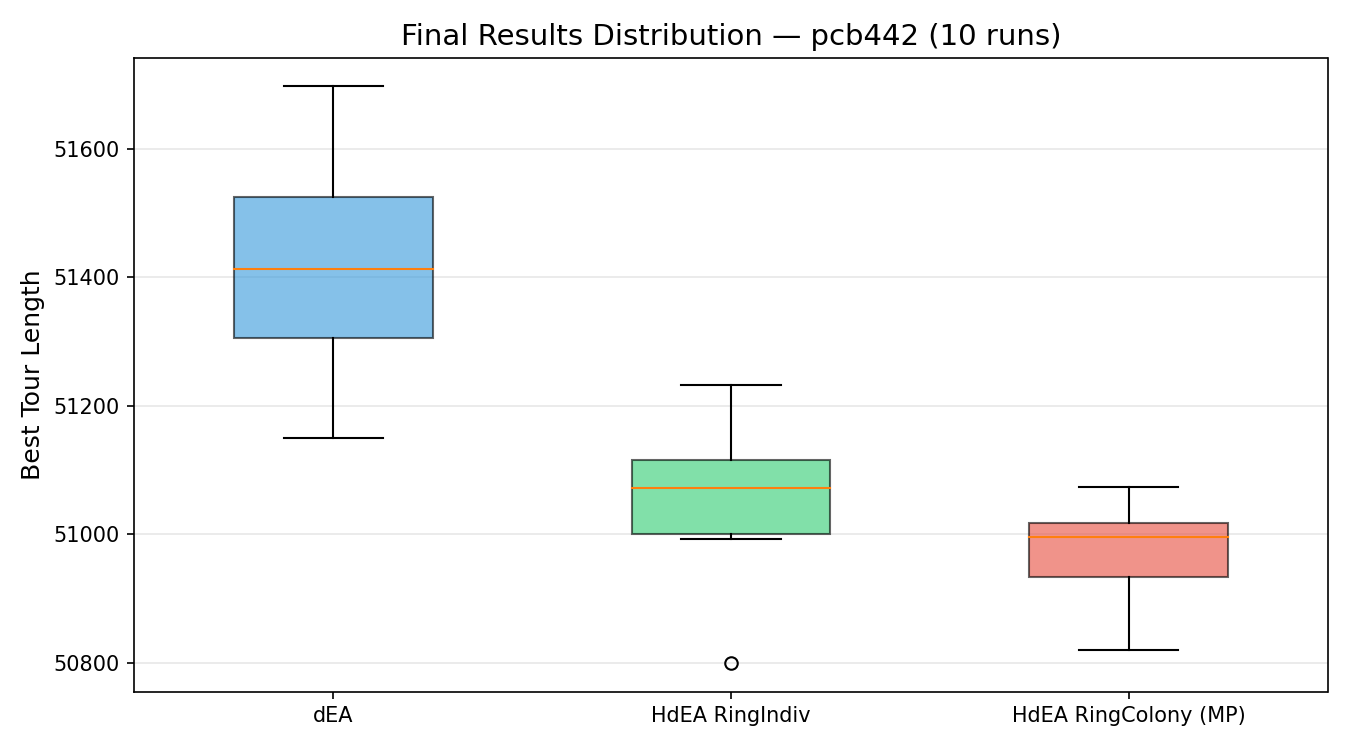
\includegraphics[width=0.85\textwidth]{boxplot.png}
\caption{箱线图：三种算法 10 次运行结果分布}
\label{fig:boxplot}
\end{figure}

\begin{figure}[H]
\centering
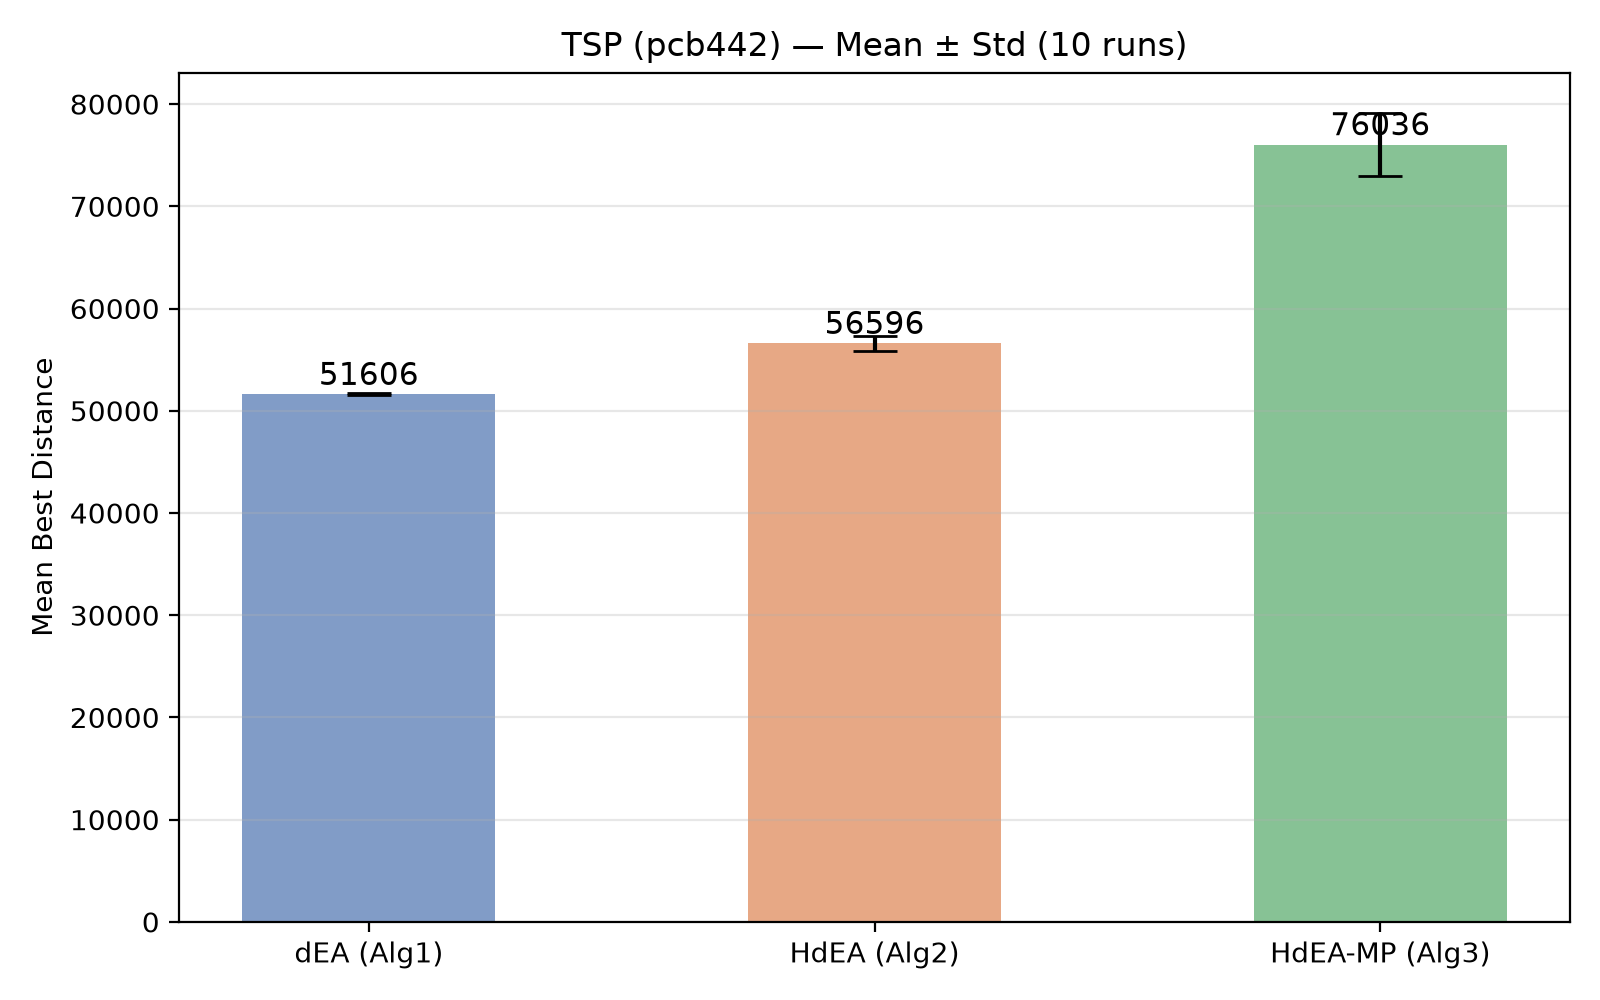
\includegraphics[width=0.85\textwidth]{barplot.png}
\caption{柱状图：三种算法均值和标准差对比（误差线表示 $\pm 1$ 标准差）}
\label{fig:barplot}
\end{figure}

\subsection{结果分析}

从实验结果可以看出，三种并行进化算法在求解质量上呈现出明显而一致的梯度：dEA 最优，HdEA 次之，HdEA-MP 最差，且两两之间的差异均通过了配对 t 检验的显著性验证（$p < 0.001$）。

dEA 以均值 51606、标准差仅 112 的成绩在求解质量上显著领先于另外两种算法。其核心优势在于全局共享种群的设计——200 个个体在同一个进化池中进行竞争、选择和交配，提供了最为充分的基因多样性，从而使种群能够持续探索搜索空间，避免陷入局部最优。从标准差来看，dEA 在 10 次运行中表现极为稳定，波动幅度（51394--51724）不超过 330，远小于 HdEA 和 HdEA-MP。

HdEA 的求解质量（均值 56596，标准差 746）明显低于 dEA，尽管其采用了更复杂的层级架构。导致这一结果的根本原因是岛屿规模过小：每个子种群仅有 50 个个体，在 442 城市的庞大搜索空间中，这一规模难以维持足够的遗传多样性。各岛屿在进化早期便快速收敛至不同的局部最优，虽然每 20 代进行一次精英迁移（将各岛最优个体汇集到 Master 再广播），但迁移仅限于最优个体的交换，对于恢复种群整体多样性的作用十分有限，最终整体最优解仍然受限于各岛屿的局部收敛质量。

HdEA-MP 的表现进一步印证了上述分析。在 HdEA 基础上增加环形迁移机制后，解质量反而出现了明显下降（均值 76036，标准差 3081）。值得注意的是，HdEA-MP 的标准差高达 3081，是三种算法中方差最大的，说明环形迁移在某些运行中确实引入了额外的基因多样性——部分运行的最优解可达到 71605。然而，由于每岛种群规模过小，迁移过来的优质基因无法在种群内有效传播和继承，最终进化结果呈现出高度的不确定性。即便是 HdEA-MP 所有运行中的最优结果（71605），也仍逊于 dEA 最差的结果（51724）。

在精度与时间这一经典权衡维度上，三种算法呈现出不同的取舍模式。dEA 每代需要两次全局集体通信（Bcast + Gatherv），通信开销约为 0.22 ms/代；HdEA 和 HdEA-MP 的大部分世代在本地独立进化，仅每 20 代进行一次通信，折合每代通信开销仅约 0.07 ms。从运行时间来看，dEA 的总耗时（约 44 s）约为 HdEA-MP（约 13 s）的 3 倍。然而 dEA 的路径距离相比 HdEA-MP 降低了约 32\%，这一解质量的提升远超额外通信所付出的时间成本。在精度优先的实际应用场景中，dEA 无疑是更为合理的选择。

\section{结论}

本报告基于 Li 与 Hu（2014）的论文框架，使用 MPI 并行编程模型完整实现了三种层次递增的分布式进化算法——Ring DEA、Ring Individual HDEA 和 Ring Colony HDEA（HdEA-MP），并以 TSPLIB 实例 pcb442 为测试平台，在 64 子种群（8×8 组）、严格遵循论文参数配置（Inver-over 算子、映射算子、临界速度机制、变异率衰减、Ring 拓扑、20:1 局部-全局比、100 全局迁移轮次）的条件下进行了系统的 10 次对比实验。

实验结果表明，两类层次化算法均以极高的统计显著性（$p<0.001$）优于基础分布式算法 dEA，其中移动种群策略的 HdEA-MP 在均值（50972）、标准差（76）和单次最优值（50821）三项指标上均为三者最优，且其运行速度约为 dEA 的两倍（347 秒对 719 秒）。层级提升的求解质量呈现出清晰的递增梯度：dEA（51409）→ HdEA（51053）→ HdEA-MP（50972），每一步升级均为求解质量带来了可量化的改善。HdEA-MP 相对于 HdEA 的优势在当前 10 次运行的样本量下尚未达到 0.05 的统计显著水平（$p=0.115$），但其在各项指标上的全面领先预示着在更大的计算规模下这一优势极有可能被统计检验所证实。

从架构层面来看，层次化迁移结构的核心价值在于：通过"微观频繁、宏观稀疏"的双层节奏设计，在子种群之间的基因交流与遗传隔离之间找到了一个平衡点，使得并行架构的独立探索优势与群体智能的信息共享需求能够同时被满足，而不会像 dEA 的扁平拓扑那样因过度交流而导致多样性过早丧失。移动种群策略则进一步深化了这一设计——将单次全局迁移的信息注入从"一个体"的量级跃升至"一个完整子种群"的量级，以边际的成本换取了质的飞跃。

本实验受限于单机 20 核的计算资源，未能以论文中的计算量（200M 代，1264 核集群）进行完整复现——两者的总计算量相差约 333 倍，这导致了本实验的绝对求解精度尚不及论文。然而，算法排名的一致性和统计显著性的稳健性充分证明了：论文中提出的架构的核心价值并不依赖于超大规模的计算资源——即使在有限资源条件下，算法设计的优劣依然是决定求解质量的主导因素。在未来的工作中，可以在更多 TSPLIB 实例（尤其是论文中的高难度实例如 u724、dsj1000 等）上扩展实验，并将子种群数扩展至论文的 64 独立物理核心配置，以获得与原始论文完全可比的求解精度。


% ---- 附录 ----
\clearpage
\section{附录：Homework 源码与说明}

本附录收录课程作业 2--6 的完整源码与设计说明。

% ===== Homework 2 =====
\subsection{Homework 2：并行归并排序}

\noindent\textbf{题目：}长度为 $m$ 的数组二分 $k$ 次，得到 $2^k$ 个子数组，每个子数组内部排序后两两归并。进程数 $n = \min(2^k, m)$，$m$ 和 $k$ 运行时输入。

\lstset{basicstyle=\scriptsize\fontspec{DejaVu Sans Mono},language=C++}
\lstinputlisting{../homework2/homework2.cpp}

\noindent\textbf{运行示例：}
\lstset{basicstyle=\scriptsize\fontspec{DejaVu Sans Mono},language={}}
\begin{lstlisting}
mpiexec -n 4 homework2.exe
m=8, k=2, needed processes=4, actual=4
Rank 0 got chunk: 3 1
Rank 0 sorted: 1 3
Rank 0 merged from rank 1, now has: 1 1 3 4
Rank 0 merged from rank 2, now has: 1 1 2 3 4 5 6 9
Final sorted array: 1 1 2 3 4 5 6 9
PASS: matches std::sort
\end{lstlisting}

\clearpage
% ===== Homework 3 =====
\subsection{Homework 3：MPI 矩阵乘法}

\noindent\textbf{题目：}利用 9 个进程并行计算 $3\times3$ 矩阵乘法 $C = A \times B$，每个进程算一个元素。

\lstset{basicstyle=\scriptsize\fontspec{DejaVu Sans Mono},language=C++}
\lstinputlisting{../homework3/homework3.cpp}

\noindent\textbf{运行示例：}
\lstset{basicstyle=\scriptsize\fontspec{DejaVu Sans Mono},language={}}
\begin{lstlisting}
mpiexec -n 9 homework3.exe
Matrix A:
   1   2   3
   4   5   6
   7   8   9
Matrix B:
   9   8   7
   6   5   4
   3   2   1
C = A x B:
  30  24  18
  84  69  54
 138 114  90
\end{lstlisting}

\clearpage
% ===== Homework 4 =====
\subsection{Homework 4：用 MPI\_Send / MPI\_Recv 实现 MPI\_Gather}

\noindent\textbf{题目：}不使用 MPI\_Gather，仅用 MPI\_Send / MPI\_Recv 实现自定义 \texttt{my\_MPI\_Gather}，并与标准 MPI\_Gather 对比验证。

\lstset{basicstyle=\scriptsize\fontspec{DejaVu Sans Mono},language=C++}
\lstinputlisting{../homework4/homework4.cpp}

\noindent\textbf{设计思路：}
\begin{itemize}
  \item root 进程先将自身数据拷贝到 recvbuf 头部。
  \item 然后按 rank 顺序接收其他进程发送的数据，写入 recvbuf 对应偏移位置。
  \item 非 root 进程各发送一个 MPI\_INT 到 root。
  \item 用标准 MPI\_Gather 的结果做校验。
\end{itemize}

\clearpage
% ===== Homework 5 =====
\subsection{Homework 5：用 MPI\_Send / MPI\_Recv 实现 MPI\_Allgather}

\noindent\textbf{题目：}不使用 MPI\_Allgather，仅用 MPI\_Send / MPI\_Recv 实现自定义 \texttt{my\_MPI\_Allgather}，并与标准 MPI\_Allgather 对比验证。

\lstset{basicstyle=\scriptsize\fontspec{DejaVu Sans Mono},language=C++}
\lstinputlisting{../homework5/homework5.cpp}

\noindent\textbf{设计思路（环形轮转）：}
\begin{enumerate}
  \item 每个进程先将自己的数据块写入 recvbuf 对应位置（rank 索引处）。
  \item 进行 $size-1$ 步环形传递：当前进程向 (rank+1) 发送一个数据块，同时从 (rank-1) 接收一个数据块。
  \item 每步目标地址由 (rank - step) mod size 计算，保证 $size-1$ 步后所有数据到达所有进程。
\end{enumerate}

\clearpage
% ===== Homework 6 =====
\subsection{Homework 6：思政思考——华为在高性能/并行计算领域的核心竞争力}

\lstset{basicstyle=\scriptsize\fontspec{DejaVu Sans Mono},language={}}
以下为思政作业原文：

\begin{lstlisting}
# 思政思考：华为在高性能/并行计算领域的核心竞争力

## 与并行计算课程的联系

华为在 HPC/并行计算领域最大的竞争力在于
"芯片—框架—编译器"全栈自研的并行计算生态，与课程内容直接对应：

| 课程概念                  | 华为对应能力                                     |
|--------------------------|------------------------------------------------|
| MPI 集体通信（Gather、Allgather、Reduce 等） | MindSpore 框架内置的分布式并行策略，自动在集群中完成梯度 Allreduce、参数 Gather 等操作 |
| 进程间通信、拓扑结构      | HCCS（华为高速互联）实现昇腾芯片间低延迟通信，类似 MPI 中 communicator 的物理层实现 |
| 并行效率、负载均衡        | 昇腾 Ascend 的达芬奇架构（DaVinci Core）专为矩阵运算并行设计，3D Cube 单元单次可完成 16x16x16 的矩阵乘加 |
| 编译器优化                | 毕昇编译器（Bisheng）针对鲲鹏/昇腾自动向量化、循环并行化 |

## 华为独特壁垒

相比 MPI 只定义"通信标准"的开放模式，华为的独特竞争力在于软硬协同：

- 鲲鹏处理器提供 ARM 架构的通用算力
- 昇腾 AI 处理器提供专用并行加速（达芬奇架构的 3D Cube）
- MindSpore 自动并行策略编排，开发者无需手动写 MPI 通信代码
- 毕昇编译器针对华为硬件深度优化

三者全栈打通，从芯片到并行框架全面自主可控。
\end{lstlisting}


\end{document}
